\chapter{Тестирование работы плагинов в тесте} \label{ch4}

% не рекомендуется использовать отдельную section <<введение>> после лета 2020 года
%\section{Введение} \label{ch4:intro}
В главе приведены результаты работы плагинов.
	
\section{Настройка Moodle} \label{ch4:sec1}

Для тестирования работы плагинов в Moodle необходимо выполнить простую установку, загрузив два архива через панель администрирования.

На \firef{fig:zip} приведён скриншот загрузки zip-архива.
\FloatBarrier % заставить рисунки и другие подвижные (float) элементы остановиться
\begin{figure}[ht] 
	\center
	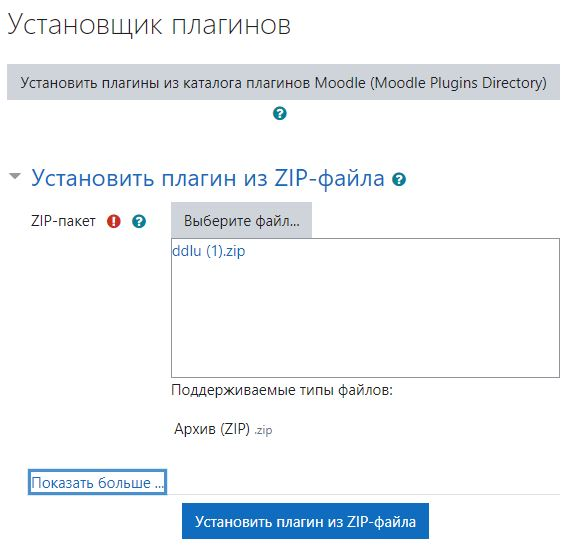
\includegraphics [scale=0.6] {my_folder/images/zip}
	\caption{Загрузка плагинов в Moodle} 
	\label{fig:zip}  
\end{figure}
\FloatBarrier % заставить рисунки и другие подвижные (float) элементы остановиться

Далее нужно создать тест, задать ему имя. Во вкладке <<Расположение>> нужно выбрать метод навигации <<Последовательный>>, в свойствах вопроса настроить режим поведения как пользовательский LusherTest, который мы загрузили ранее. Далее перейдём на вкладку <<Настройки просмотра>>, где уберём все галочки, связанные с баллами и правильными ответами, так система оценивания Moodle не подходит для нашего теста.

На \firef{fig:set1} приведён скриншот с настройками расположения и свойств вопросов.
На \firef{fig:set2} приведены настройки просмотра результатов.
\FloatBarrier % заставить рисунки и другие подвижные (float) элементы остановиться
\begin{figure}[ht] 
	\center
	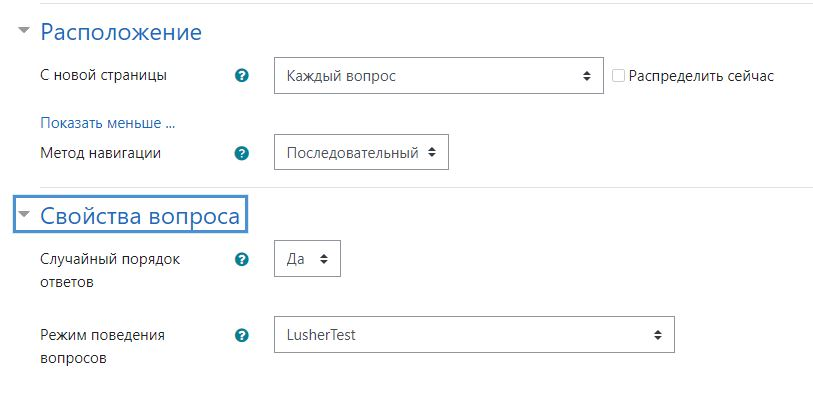
\includegraphics [scale=0.5] {my_folder/images/setting1}
	\caption{Настройки пунктов <<Расположение>> и <<Свойства вопроса>>} 
	\label{fig:set1}  
\end{figure}
\FloatBarrier % заставить рисунки и другие подвижные (float) элементы остановиться
\FloatBarrier % заставить рисунки и другие подвижные (float) элементы остановиться
\begin{figure}[ht] 
	\center
	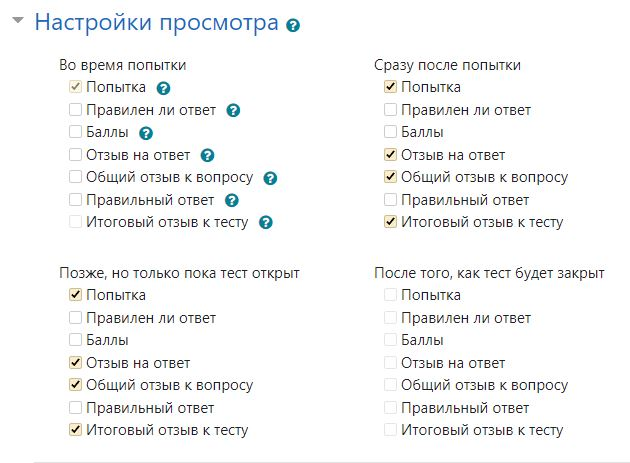
\includegraphics [scale=0.7] {my_folder/images/setting2}
	\caption{Настройки просмотра} 
	\label{fig:set2}  
\end{figure}
\FloatBarrier % заставить рисунки и другие подвижные (float) элементы остановиться
В тесте было создано 2 вопроса загруженного нами типа.

\section{Тестирование работы} \label{ch4:sec2}

После запуска теста на экране появились все карточки и кнопка продолжения, которая не работает, если цвета не перенесены на фоновое изображение. Панель навигации видна, но не работает, как и следовало ожидать. Карточки при перетаскивании исчезали. Исчезновение карточек приведено на \firef{fig:test1}.

\FloatBarrier % заставить рисунки и другие подвижные (float) элементы остановиться
\begin{figure}[ht] 
	\center
	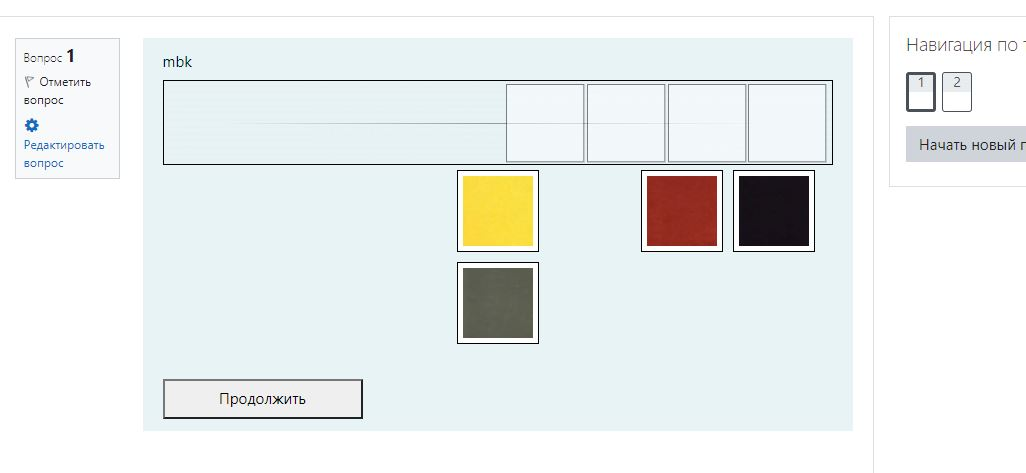
\includegraphics [scale=0.5] {my_folder/images/test1}
	\caption{Исчезновение карточек} 
	\label{fig:test1}  
\end{figure}
\FloatBarrier % заставить рисунки и другие подвижные (float) элементы остановиться

Между вопросами запустился таймер, по истечении времени которого стала доступна кнопка перехода ко второму вопросу. На \firef{fig:time} отображена страница с таймером.
\FloatBarrier % заставить рисунки и другие подвижные (float) элементы остановиться
\begin{figure}[ht] 
	\center
	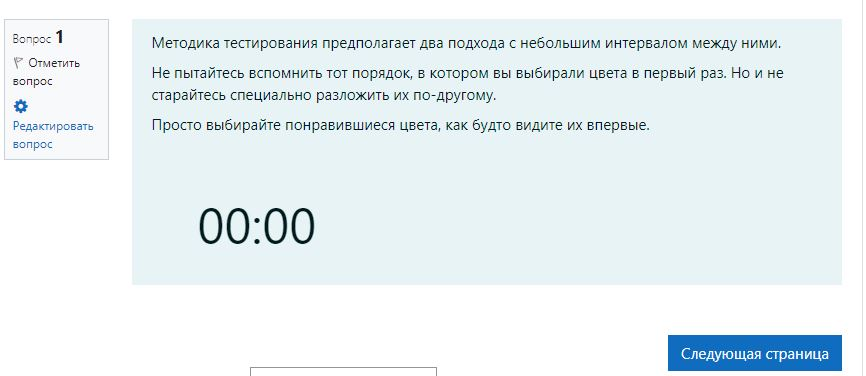
\includegraphics [scale=0.7] {my_folder/images/between}
	\caption{Таймер между вопросами} 
	\label{fig:time}  
\end{figure}
\FloatBarrier % заставить рисунки и другие подвижные (float) элементы остановиться

Тест успешно завершился и показал предварительную оценку тревожности. На \firef{fig:res1} и \firef{fig:res2} можно увидеть страницу отображения результатов теста.
\FloatBarrier % заставить рисунки и другие подвижные (float) элементы остановиться
\begin{figure}[ht] 
	\center
	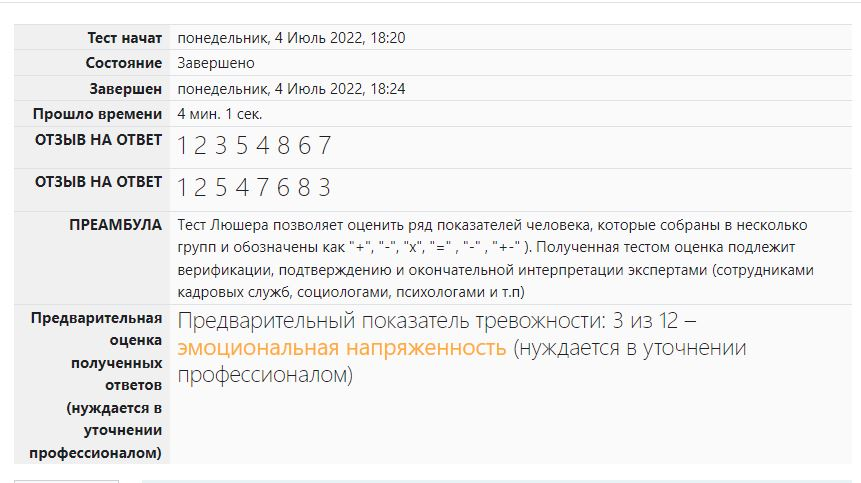
\includegraphics [scale=0.7] {my_folder/images/restest1}
	\caption{Оценка тревожности} 
	\label{fig:res1}  
\end{figure}
\FloatBarrier % заставить рисунки и другие подвижные (float) элементы остановиться

\FloatBarrier % заставить рисунки и другие подвижные (float) элементы остановиться
\begin{figure}[ht] 
	\center
	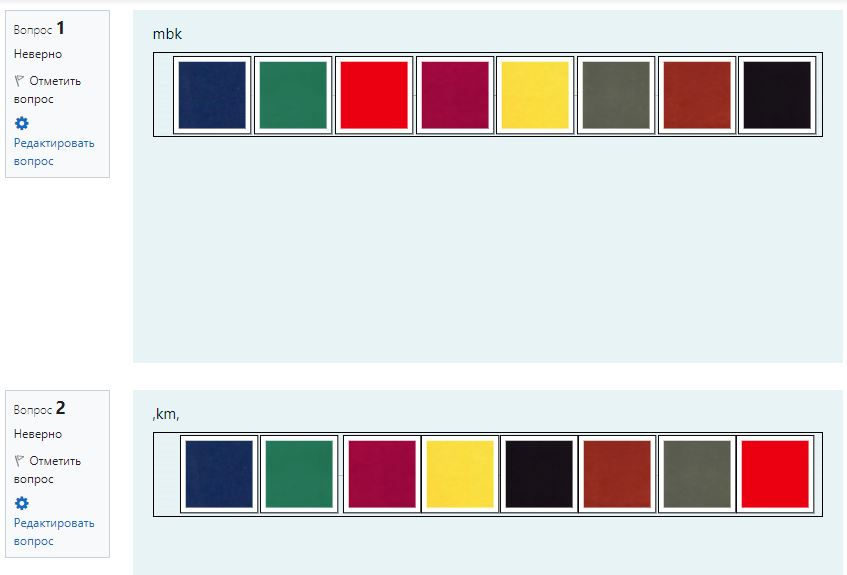
\includegraphics [scale=0.7] {my_folder/images/restest2}
	\caption{Отображение карточек в результатах} 
	\label{fig:res2}  
\end{figure}
\FloatBarrier % заставить рисунки и другие подвижные (float) элементы остановиться
%Пример ссылки на литературу \cite{avtonomova:fya,Peskov2004-ru,Kotelnikov2004-ru,Kotelnikov2004}.

%\FloatBarrier % заставить рисунки и другие подвижные (float) элементы остановиться

%\section{Выводы} \label{ch4:conclusion}

%Текст выводов по главе \thechapter.

%% Вспомогательные команды - Additional commands
%
\newpage % принудительное начало с новой страницы, использовать только в конце раздела
%\clearpage % осуществляется пакетом <<placeins>> в пределах секций
%\newpage\leavevmode\thispagestyle{empty}\newpage % 100 % начало новой страницы